\documentclass{bnmcvdc}

\usepackage[spanish]{babel}
\usepackage[ansinew]{inputenc}
\usepackage{enumerate}
\usepackage[newitem,newenum]{paralist}
\usepackage{url}
\usepackage{pdfpages}

\newboolean{ingles}
\setboolean{ingles}{false}
\newcommand{\bi}[2]{\ifthenelse{\boolean{ingles}}{#1}{#2}}

\renewcommand{\labelitemi}{\rule[2pt]{2.5pt}{2.5pt}}
\renewcommand{\labelitemii}{\rule[2.5pt]{1.5pt}{1.5pt}}
\renewcommand{\labelitemiii}{-}
\renewcommand\labelitemiv{\textperiodcentered}

%%%%%%%%%%%%%%%%%%%%%%%%%%%%%%%%%%%%
\newcommand{\inputpath}{src/}
%%%%%%%%%%%%%%%%%%%%%%%%%%%%%%%%%%%%
\newcommand{\depto}{COMPUTACI\'ON}
\newcommand{\condicion}{Concurso }
%\newcommand{\condicion}{Selecci\'on Interina }
\newcommand{\cargo}{Asociado}
\newcommand{\dedicacion}{Exclusiva}
%\newcommand{\dedicacion}{Semiexclusiva}
%\newcommand{\dedicacion}{Parcial}
%\newcommand{\area}{Ingenier\'ia de Software}
\newcommand{\area}{s/a}
%\newcommand{\area}{Cs. Exactas y Naturales}
%\newcommand{\campoinv}{-}
\newcommand{\campoinv}{}
\newcommand{\expediente}{505.705/15}%cambiar!!
\newcommand{\linea}{\rule{14.5cm}{0.2mm}}
\newcommand{\comment}[1]{}
\newcommand{\firma}{
\vfill

\hspace{8cm} \dotfill

\hspace{10.5cm}Firma
\begin{flushright}
{\scriptsize $\quad$}
\end{flushright}
\newpage}
\newcommand{\firmb}{
\vfill

\hspace{8cm} \dotfill

\hspace{10.5cm}Firma
\begin{flushright}
{\scriptsize Se anexa una p\'agina a continuaci\'on.  $\mapsto$}
\end{flushright}
\newpage}
\newcommand{\firmc}[1]{
\vfill

\hspace{8cm} \dotfill

\hspace{10.5cm}Firma
\begin{flushright}
{\scriptsize Se anexan #1 p\'aginas a continuaci\'on. $\mapsto$}
\end{flushright}
\newpage}
%%%%%%%%%%%%%%%%%%%%%%%%%%%%%%%%%%%%

\oddsidemargin 0.5cm \topmargin -0.7in \textwidth 14.5cm
\textheight 10in
\parskip 6pt
\parindent=0cm

\begin{document}

\fuente

~

\vspace{.5cm}

\begin{center}

{\large \textbf{Leandro Ezequiel Nahabedian}} \\

\bigskip

%Actualizaci\'on de Curriculum Vitae al \today \\

\condicion Expte. Nro. \expediente  \\ % DC

\end{center}

\bigskip

\section*{\espacio Datos Personales}

\begin{itemize}


\end{itemize}


\section*{\espacio Posici\'on actual}

\begin{itemize}

    
%\item Jefe de Trabajos Pr\'acticos regular con 
%dedicaci\'on exclusiva
%    del Departamento de Computaci\'on de la Facultad de 
%    Ciencias
%    Exactas y Naturales de la Universidad de Buenos Aires.
%    (en uso de licencia).

%\item Jefe de Trabajos regular \'area Teor\'ia con
%    dedicaci\'on
%    parcial del Departamento de Computaci\'on de la Facultad de Ciencias
%    Exactas y Naturales de la Universidad de Buenos Aires 
%    (en uso de licencia).

%\item Investigador Asistente en la Carrera del Investigador
%Cient\'{\i}fico y Tecnol\'ogico del CONICET, \'area 
%Computaci\'on, (recib\'i correo confirmando mi ingreso en 
%el 
%d\'ia de la fecha).

%\item Secretario Acad\'emico del Departamento de Computaci\'on de la Facultad de 
%    Ciencias Exactas y Naturales de la Universidad de Buenos Aires. 
%    Desde julio de 2012.

%\item Consejero Directivo representante de la mayor�a del claustro de graduados. 
%    Desde marzo de 2014.

\end{itemize}

\newpage


%PAGINA 2
A.~TITULOS UNIVERSITARIOS OBTENIDOS (indicando Facultad,
Universidad y fecha que se ha expedido)

\vskip 1cm

\begin{itemize}
\item Doctorando en Ciencias de la Computaci\'on.
    \begin{compactitem}[-]
        \item Instituci\'on: Universidad de Buenos Aires
        \item Fecha de Egreso: Diciembre de 2019 (esperado)
        \item Tesis: ``Adaptaci\'on v\'ia Controladores Discretos Multi-Capa''
        \item Directores: Dr. Sebasti\'an Uchitel
\end{compactitem}

\item Licenciado en Ciencias de la Computaci\'on.
    \begin{compactitem}[-]
        \item Instituci\'on: Facultad de Ciencias Exactas y Naturales
    (Universidad de Buenos Aires)
        \item Fecha de Egreso: Diciembre de 2014
%        \item Promedio: 7,80
        \item Tesis de licenciatura: ``Hot-Swap: Una t\'ecnica para la generaci\'on y actualizaci\'on autom\'atica de controladores discretos en tiempo de ejecuci\'on''
        \item Director: Dr. Nicol\'as D'Ippolito
\end{compactitem}

%\medskip
\item T\'{\i}tulo secundario: Perito en T\'ecnicas Bancarias e Impositivas.
    \begin{compactitem}[-]
    	\item Instituto Ana Mar\'ia Janer.
	\item Fecha de Egreso: 2006
    \end{compactitem}

\end{itemize}


\newpage


%PAGINA 3

B.~ANTECEDENTES DOCENTES E INDOLE DE LAS TAREAS DESARROLLADAS (indicando instituci\'on, per\'iodo de ejercicio y naturaleza de su designaci\'on, lapso y lugar en que fueron realizados)

\subsection*{Universitarios}

\begin{compactitem}
%\item[Junio 2016 - a la fecha] Profesor Adjunto Regular \'area 
%Sistemas o Ingenier\'ia de Software o Programaci\'on dedicaci\'on
%    parcial del Departamento de Computaci\'on de la Facultad de
%    Ciencias Exactas y Naturales (UBA).

%\item[Marzo 2013 - Mayo 2016] Profesor Adjunto interino area 
%Ingenier\'ia de Software con 
%    dedicaci\'on
%    simple del Departamento de Computaci\'on de la Facultad de
%    Ciencias Exactas y Naturales (UBA).

%\item[Marzo 2012 - Marzo 2013] Jefe de Trabajos
%    Pr\'acticos interino area Ingenier\'ia de Software con     dedicaci\'on
%    simple del Departamento de Computaci\'on de la Facultad de
%    Ciencias Exactas y Naturales (UBA).
    
%\item[Julio de 2011 - Marzo 2013] Jefe de Trabajos
%    Pr\'acticos interino area Ingenier\'ia de Software con dedicaci\'on
%    exclusiva del Departamento de Computaci\'on de la Facultad de Ciencias Exactas y Naturales (UBA) 

%\item[2011-2012] \bi{Course Leader}{Jefe
%    de Trabajos Pr\'acticos}\\
%    \bi{\emph{Concurrecy} course\\Computing Department Imperial
%    College London}{Materia ``Concurrencia'' (Concurrency). Materia obligatoria del curr\'iculo del MSc.\\ Computing Department, Imperial
%    College London\\ Breve
%descripci\'on: La materia cubre conceptos, m\'etodos y algoritmos
%para la construcci\'on de programas concurrentes
%(\url{http://www.doc.ic.ac.uk/teaching/coursedetails/223}).}
%
%\item[2008 - 2010] \bi{Teaching assistant}{Ayudante de
%    c\'atedra}.\\
%    \bi{Course: Concurrency. Computing Department, Imperial College London}{Materia
%    ``Concurrencia'' (Concurrency)\\
%    Computing Department, Imperial College London}.



%\medskip
%
%\bi{}{ \subsection*{\bi{}{Resumen de cuatrimestres}}
%\begin{center}
%\begin{tabular}{|c|c|c|}
%  \hline
%  % after \\: \hline or \cline{col1-col2} \cline{col3-col4} ...
%  Cargo & Dedicaci\'on & Cuatrimestres\\
%  \hline
%  PAD & Parcial & 2\\
%  JTP & Parcial & 3\\
%  Ay. $\fuente 1^{a}$ & Exclusiva & 9 \\
%  Ay. $\fuente 1^{a}$ & Parcial & 2 \\
%  Ay. $\fuente 2^{a}$ & Parcial & 4 \\
%  Ay. Ad Honorem & Parcial & 2 \\
%  \hline
%\end{tabular}
%\end{center}
%}

\end{compactitem}

%\subsection*{\bi{Non-university teaching}{Experiencia docente no
%universitaria}}
%\begin{compactitem}
%\item[2006 - 2008] \bi{IT Training Center - Upper Bound.
    Instructor of official Sun Microsystems and IBM courses JAVA
    and J2EE courses.}{IT Training Center - Upper Bound.
    Instructor de cursos JAVA y J2EE Sun Microsystems e IBM
    oficiales.}

%\end{compactitem}


\subsection*{Primarios y secundarios}

\begin{compactitem}
\item Desde Marzo hasta noviembre de 2009 dict\'e clases de apoyo a estudiantes de colegio secundario. Dichas clases eran de matem\'atica, f\'isica e ingl\'es. Estos estudiantes concurr\'ian a colegios especiales para completar sus estudios secundarios. 

\end{compactitem}

%\subsection*{Publicaciones relacionadas con la docencia}
%
%\begin{compactitem}
%
\item   Bonomo F., D'Andrea C., Laplagne S., Szew M., ``Explorando
la geometr\'{\i}a en los Clubes Cabri'', editorial Red
Ol\'{\i}mpica, Argentina, 1996, ISBN 987-9072-15-4, 140 p\'aginas.

\item   Bonomo F., Laplagne S., Szew M., Tilli D., ``Competencias
entre Clubes Cabri'', editorial Red Ol\'{\i}mpica, Argentina,
1999, ISBN 987-9072-25-1, 135 p\'aginas.

%\end{compactitem}




\newpage
%PAGINA 4

C.~ANTECEDENTES CIENT\'IFICOS%, CONSIGNANDO LAS PUBLICACIONES
%(identificar a los autores, indicar editorial o revista, lugar y
%fecha de publicaci\'on, volumen, n\'umero y p\'aginas) U OTROS
%RELACIONADOS CON LA ESPECIALIDAD (indicando lapso y lugar en que
%fueron realizados).

%   Si se invocasen trabajos in\'editos deber\'a presentar un ejemplar
%   firmado por el aspirante, el que ser\'a agregado al expediente
%   del concurso.

%\subsection*{Trabajos publicados o en prensa en revistas internacionales indexadas (ISI)}

%\begin{compactenum}
%%\subsection*{Trabajos publicados o en prensa en revistas internacionales indexadas (ISI)}

%\item {\footnotesize Sebasti�n Uchitel, Dalal Alrajeh, Shoham Ben-David, V�ctor A. Braberman, Marsha Chechik, Guido de Caso,  \underline{Nicol\'as D'Ippolito}, Dario Fischbein, Diego Garbervetsky, Jeff Kramer, Alessandra Russo, German E. Sibay}\\
% \textbf{Supporting incremental behaviour model elaboration}\\
%{\em Computer Science - Research and Development},  28(4): 279-293 (2013).\\
%{\small \bi{}{Relevancia: Paper invitado por los editores de CSRD.}}

%\item {\footnotesize \underline{Nicol\'as D'Ippolito}, Victor Braberman, Nir Piterman, Sebasti\'an Uchitel}\\
% \textbf{Synthesising Non-Anomalous Event-Based Controllers
% for Liveness Goals}
% \\
%{\em ACM Transactions on Software Engineering and Methodology},
%22(1): 9 (2013).\\
%(\bi{Impact factor in}{Factor de impacto en} 2008: 3.58)\\
%{\small \bi{}{Relevancia: en este trabajo adaptamos y extendemos el trabajo presentado en FSE 2010. No solo extendimos varias de las secciones existentes, sino que tambi\'en agregamos secciones nuevas,
%como ser la de implementaci\'on. Asimismo, mejoramos la presentaci\'on en general agregando intuiciones y ejemplos.}}

%\item {\footnotesize Dario Fischbein, Greg Brunet, \underline{Nicol\'as D'Ippolito}, Marsha Chechik, Sebasti\'an Uchitel}\\ 
%\textbf{Weak Alphabet Merging of Partial Behaviour Models}\\
%{\em ACM Transactions on Software Engineering and Methodology}, 21(2): 9 (2012).\\
%(\bi{Impact factor in}{Factor de impacto en} 2008: 3.58)\\
% {\small \bi{}{Relevancia: en este paper proponemos la sem\'antica ``weak alphabet'' como respuesta a algunas de las preguntas fundamentales en el mundo de los modelos de comportamiento
%parcial. Definimos formalmente el ``merge'' de moledos y estudiamos propiedades algebraicas de la composici\'on en paralelo de modelos parciales MTS. Este trabajo es anterior al comienzo de mi doctorado y est\'a fuertemente relacionado con los temas desarrollados en mi tesis de licenciatura.} }

%\end{compactenum}


%\subsection*{Trabajos publicados o en prensa en revistas regionales con referato internacional}


%\subsection*{Trabajos publicados en otras revistas internacionales o regionales con referato}
%
%\begin{compactenum}
%\item Bonomo F. and Dur\'an G., ``Computational complexity of
classical problems for hereditary clique-Helly graphs'', Pesquisa
Operacional 24(3) (2004), 435--443.

%\end{compactenum}

%\subsection*{Cap\'{\i}tulos de libros}

%\begin{compactenum}
%
\item {\footnotesize Victor Braberman, \underline{Nicol\'as D'Ippolito}, Jeff Kramer, Daniel Sykes, and Sebastian Uchitel}\\ 
\textbf{An extended description of MORPH: A Reference Architecture for Configuration and Behaviour Self-Adaptation}\\
{\em Software Engineering for Self-Adaptive Systems: A Third Research Roadmap (2016).}\\
%(\bi{Impact factor in}{Factor de impacto en} 2008: 3.58)\\
% {\small \bi{}{Relevancia: en este paper proponemos la sem\'antica ``weak alphabet'' como respuesta a algunas de las preguntas fundamentales en el mundo de los modelos de comportamiento
%parcial. Definimos formalmente el ``merge'' de moledos y estudiamos propiedades algebraicas de la composici\'on en paralelo de modelos parciales MTS. Este trabajo es anterior al comienzo de mi doctorado y est\'a fuertemente relacionado con los temas desarrollados en mi tesis de licenciatura.} }

%\end{compactenum}


\subsection*{Trabajos publicados en actas de congresos
internacionales con referato}

%%%%%%%%aclarar que congreso y donde esta el paper completo


\begin{compactenum}





\end{compactenum}


%\firmb

\subsection*{Posters}


\begin{compactenum}


\end{compactenum}


%\subsection*{Trabajos enviados para su publicaci\'on}

%\begin{compactenum}
%%\item Leandro Nahabedian, Victor Braberman, \underline{Nicol\'as D'Ippolito}, Shinichi Honiden, Jeff Kramer, Kenji Tei, Sebasti\'an Uchitel\\
% \textbf{Forcing Assured Dynamic Controller Update?}\\
%Enviado a la 38th International Conference on Software Engineering Austin, TX, May 14 - 22, 2016 (ICSE'16).


%\end{compactenum}


%\subsection*{Participaci\'on en proyectos de investigaci\'on financiados}

%\textbf{$\quad$ Actuales}


%\begin{compactitem}
%\item[2014 - 2016]\textbf{Financiamiento para proyectos de investigaci�n del  Instituto de Investigaciones Cient�ficas y T�cnicas para la Defensa (CITEDEF), Ministerio de Defensa de la Naci�n Argentina)}\\
``Proyecto: Sistema de A\'ereo No Tripulado''\\
\bi{Principal Investigator}{Investigador Responsable}: Dr. Nicol�s D'Ippolito\\
Monto Financiado: 3.700.000\$.\\
%Descripci\'on: El objetivo de este proyecto es el desarrollo de un sistema a\'ereo no tripulado (SANT) integrado por un conjunto de veh\'iculos y una estaci\'on de monitoreo y control de misiones. El desarrollo abarca el dise\~no integral del sistema desde las componentes de hardware hasta el soporte de software. Este proyecto est\'a enmarcado en una propuesta cient\'ifico tecnol\'ogica que involucra no s\'olo el desarrollo del producto sino tambi\'en un ACCAAAAAAAA
%
\item[2014 - 2016]\textbf{Convocatoria PIDDEF 2014-2017}\\
``Proyecto: Sistema de A\'ereo No Tripulado''\\
\bi{Principal Investigator}{Investigador Responsable}: Dr. Nicol�s D'Ippolito\\
Monto Financiado: \$ 5.000.000.\\

\item[2014 - 2017]\textbf{Convocatoria UBACyT-Programaci\'on Cient\'ifica (2014-2017)}\\ 
``S�ntesis de Controladores para la Ingenier�a de Software''\\
\bi{Principal Investigator}{Investigador Responsable}: Dr. Nicol�s D'Ippolito.\\

\item[2011 - 2014] \textbf{UBACYT  20020100100813}
``Modelos formales en la ingenier�a de software: construcci�n, validaci�n y verificaci�n''\\
Investigador Responsable: Sebasti�n Uchitel\\

\item[2013-2016] \textbf{PICT 2012 N� 0724}\\
``Behavior Abstractions for Software Testing''\\
Investigador Responsable:  V�ctor Braberman\\

\item[2012 - 2015]\textbf{Pr�stamo BID - PICT 2011 1774 (2012 � 2015)}\\
``S�ntesis de Controladores para la Ingenier�a de Software''\\
\bi{Principal Investigator}{Investigador Responsable}: Dr. Sebasti\'an Uchitel.\\

\item[2011-2015] \textbf{FP7-PEOPLE-2011-IRSES}\\
``MEALS: Mobility between Europe and Argentina applying Logics to System''\\
Investigadores Responsables: Holger Hermans / Pedro D'Argenio\\

%\end{compactitem}

%\textbf{$\quad$ Finalizados}

%\begin{compactitem}
%\item[2007 - 2013] \textbf{UBACYT X021}\\
``An�lisis din�mico y est�tico de aplicaciones y modelos''\\
\bi{Principal Investigator}{Investigador Responsable}: Dr. Victor
Braberman.\\

\item[2007 - 2013]\textbf{PAE-PICT 2007-02272}\\
``Modelado de sistemas tolerantes a fallas''\\
\bi{Principal Investigator}{Investigador Responsable}: Dr. Sebasti\'an
Uchitel.\\

\item[2007 - 2013] \bi{Project}{Proyecto}: ``Partial Behaviour
    Modelling:     A Foundation for Incremental and Iterative
    Model-Based Software Engineering''\\
    \bi{Funding}{Financiamiento}: European Research Council
    (ERC 204853/PBM). \\
    Investigador Responsable: Dr. Sebasti\'an
    Uchitel. \\ %(Imperial College London/University of Buenos Aires).\\

\item[2011-2013] \textbf{PICT 2010 N�02351}\\
``An�lisis cuantitativo del uso de la memoria din�mica con foco en la escalabilidad y usabilidad''\\
Investigador Responsable: Diego Garbervetsky\\
%\end{compactitem}

%\newpage
\vspace{1cm}
%
D.~CURSOS DE ESPECIALIZACI\'ON SEGUIDOS, CONFERENCIAS Y TRABAJOS DE INVESTIGACI\'ON REALIZADOS SEAN ELLOS EDITOS O INEDITOS (indicando lapso y lugar en que fueron realizados).

%{\small Si se invocasen trabajos in\'editos deber\'a presentar un ejemplar firmado por el aspirante, el que \underline{ser\'a agregado} al expediente del concurso.}


\subsection*{Charlas dictadas por invitaci\'on o en seminarios}

\begin{compactitem}
\item[Marzo 2015]
Disertante\\  Tercer Taller Argentino de Fundamentos para el An\'alisis y Construcci\'on Autom\'atica de Software. FACAS 2015.\\
``Assured and Correct Dynamic Controller Update''

\item[Noviembre 2014]
Disertante\\ 2do Workshop Internacional UBA-NII.\\
``Forzing Dynamic Controller Update''

\end{compactitem}

%\pagebreak

\subsection*{Asistencia a cursos, escuelas y congresos}

\begin{compactitem}
\item[2012] Generaci�n Autom�tica de Tests Unitarios\\
    \bi{In}{En} ECI 2012\\
    \bi{Tutor}{Docente}: Nazareno Aguirre\\
    \bi{Length}{Duraci\'on}: 20hs


\end{compactitem}


%\firmb


\vspace{1cm}
\newpage

E.~1-ACTUACI\'ON EN UNIVERSIDADES E INSTITUTOS NACIONALES, PROVINCIALES Y PRIVADOS REGISTRADOS EN EL PAIS O EN EL EXTERIOR

%\vspace{1cm}

%\subsection*{Cargos de gesti\'on}

%\begin{compactitem}
%\item[desde 2014] Consejero Directivo. Representante de graduados por la mayor\'ia.

\item[Julio 2012 - Octubre 2014] Secretario Acad\'emico del Departamento de
    Computaci\'on de la FCEyN, UBA.

\item[Marzo 2012 - Marzo 2014] Consejero Departamental del Departamento de
    Computaci\'on de la FCEyN, UBA, por el claustro de graduados.

\item[desde 2011] Integrante de la Comisi\'on de Ense\~nanza del Consejo Directivo\\
        Representante de la mayor\'ia de Graduados  \\
         FCEyN, Universidad de Buenos Aires.

\item[2011] Colaborador de la organizaci\'on\\
      Escuela de Ciencias Inform\'aticas 2011\\
    Departamento de Computaci\'on\\
    FCEyN, Universidad de Buenos Aires.

\item[2010] Miembro de la organizaci\'on\\
      Reuni\'on de Graduados 2010\\
    Departamento de Computaci\'on, FCEyN, Universidad de Buenos
    Aires

%\end{compactitem}

%\newpage

\vspace{1cm}


2- CARGOS QUE DESEMPENO O DESEMPENA EN LA ADMINISTRACI\'ON P\'UBLICA O
EN LA ACTIVIDAD PRIVADA, EN EL PAIS O EN EL EXTRANJERO (indicando
organismo o entidad, lugar y lapso)
%
%
%%\subsection*{Cargos de investigaci\'on}
%%
%%\begin{compactitem}
%%
\item Investigadora Asistente en la Carrera del Investigador
Cient\'{\i}fico y Tecnol\'ogico del CONICET, \'area Matem\'atica y
Computaci\'on, desde marzo de 2007.

%%\end{compactitem}
%
%
\subsection*{Estad\'{\i}as de investigaci\'on en el exterior por invitaci\'on}

\begin{compactitem}
\item[\bi{March}{Marzo} 2014 - Junio 2014] National Institute of Informatics,Tokio Jap\'on.\\
    \bi{Invited by}{Colaborador}: Prof. Kenji Tei.\\
    \bi{Funding}{Financiamiento}: National Institute of Informatics.


\end{compactitem}

\subsection*{Becas de investigaci\'on y pasant\'{\i}as}

\begin{compactitem}



\end{compactitem}


%\vspace{1cm}
\newpage

F.~PARTICIPACI\'ON EN CONGRESOS O ACONTECIMIENTOS SIMILARES NACIONALES O INTERNACIONALES
%(indicando lugar y lapso en que se realizaron y calidad de representaci\'on).

\vspace{.5cm}

\textbf{$\quad$ Internacionales}

\smallskip

\begin{compactitem}
\item[2016] ICSE - International Conference of  Software Engineering\\
\bi{Main Conference}{Conferencia principal}

\item[2016] SEAMS - Symposium on Software Engineering for Adaptive and Self-Managing Systems\\
    \bi{Presentation}{Trabajo presentado}:
``Assured and Correct Dynamic Update of Controllers''

\end{compactitem}

\bigskip



%\textbf{$\quad$ Regionales}
%
%\smallskip
%
%\begin{compactitem}
%\item Octubre 2008, Guanajuato, Mexico - Tercer Taller
Latinoamericano de Clanes en Gr\'aficas. Trabajos presentados:
\begin{compactitem}
\item[-] Bonomo F. and Cerioli M.R., ``On $L(2,1)$-labeling of
block graphs'' \item[-] Bonomo F., Dur\'an G., Safe M.D. and
Wagler A.K., ``Partial characterizations of balanced graphs''.
\end{compactitem}

\smallskip

\item Noviembre 2007, P. Montt, Chile - VII Congreso Chileno de
Investigaci\'on Ope\-ra\-ti\-va (OPTIMA). Semi-plenaria invitada:
\begin{compactitem}
\item[-] ``Introducci\'on a las redes complejas''.
\end{compactitem}

\smallskip

\item Noviembre 2006, Montevideo, Uruguay - XIII Latin-Iberian
American Congress of Operations Research (CLAIO). Trabajo
presentado:
\begin{compactitem}
\item[-] Bonomo F., Dur\'an G. and Marenco J., ``Exploring the
complexity boundary between coloring and list coloring''.
\end{compactitem}

\smallskip


\item Octubre 2006, La Plata - II Workshop Latino-Americano de
Cliques en Grafos. Comunicaciones presentadas:
\begin{compactitem}
\item[-] Bonomo F., Dur\'an G. and Marenco J., ``Exploring the
complexity boundary between coloring and list coloring'' \item[-]
Bonomo F., ``Self-clique Helly circular-arc graphs''.
\end{compactitem}

\smallskip

\item Febrero 2004, Montevideo, Uruguay - IX Escuela
Latinoamericana de Verano de Investigaci\'on Operativa (ELAVIO).
%Latin American Summer School of Operations Research
Comunicaci\'on presentada:
\begin{compactitem}
\item[-] Bonomo F., Dur\'an G., Lin M. and Szwarcfiter J., ``On
balanced graphs''.
\end{compactitem}

\smallskip

\item Septiembre 2003, Valpara\'{\i}so, Chile - V Congreso Chileno
de Investigaci\'on Ope\-ra\-ti\-va (OPTIMA). Trabajo presentado:
\begin{compactitem}
\item[-] Bonomo F., Dur\'an G. and Groshaus M., ``Coordinated
graphs and clique graphs of clique-Helly perfect graphs''.
\end{compactitem}

\smallskip

\item Febrero 2003, Vaquer\'{\i}as, Argentina - VIII Escuela
Latinoamericana de Verano de Investigaci\'on Operativa (ELAVIO).
Comunicaci\'on presentada:
\begin{compactitem}
\item[-] Bonomo F. y Dur\'an G., ``La complejidad computacional de
algunos proble\-mas cl\'asicos en grafos clique-Helly
hereditarios, perfectos y K-perfectos''.
\end{compactitem}

\smallskip

\item Octubre 2002, Concepci\'on, Chile - XI Latin-Iberian
American Congress of Operations Research (CLAIO). Trabajos
presentados:
\begin{compactitem}
\item[-] Bonomo F., Dur\'an G. and Groshaus M., ``On
clique-perfect, coordinated and K-perfect graphs'' \item[-] Bonomo
F., Dur\'an G. and Groshaus M., ``Computational Complexity of some
Classical Problems on Hereditary Clique-Helly Graphs''.
\end{compactitem}

\smallskip

\item Abril 2002, Rio de Janeiro, Brasil - Workshop
Latino-Americano de Cliques em Grafos. Comunicaciones presentadas:
\begin{compactitem}
\item[-] Bonomo F., Dur\'an G. and Groshaus M., ``On
clique-perfect, K-perfect and coordinated graphs'' \item[-] Bonomo
F., Dur\'an G., Lin M. and Szwarcfiter J., ``On Cliques of
Balanced Graphs''.
\end{compactitem}

%\end{compactitem}
%
%\bigskip
%
%\textbf{$\quad$ Nacionales}
%
%\smallskip
%
%\begin{compactitem}
%\item Septiembre 2014, Buenos Aires - 43 JAIIO - Simposio Argentino de
Ingenier\'ia de Software (ASSE). Trabajo presentado:
\begin{compactitem}
\item[-] ``Hope for the best, prepare for the worst: multi-tier control for adaptive systems'.
\end{compactitem}

\item Septiembre 2014, Buenos Aires - 43 JAIIO - Simposio Argentino de
Ingenier\'ia de Software (ASSE). Trabajo presentado:
\begin{compactitem}
\item[-] ``Revisiting Compatibility of Input-Output Modal Transition Systems'.
\end{compactitem}




%\end{compactitem}
%

%\pagebreak

\subsection*{Actuaci\'on en comit\'es de reuniones cient\'{\i}ficas}

\begin{compactitem}
\item Asistente del Cuarto Taller Argentino de Fundamentos para el An�lisis y Construcci�n Autom�tica de Software - FACAS 2016 

\item Subreviewer de Nicol\'as D'Ippolito del Tool Track de la 10th Joint Meeting of the European Software Engineering Conference and the ACM SIGSOFT Symposium on the Foundations of Software - ESEC/FSE 2015.

\item Subreviewer de Nicol\'as D'Ippolito de First International Workshop on Control Theory for Software Engineering - CTSE 2015. Workshop sat\'elite de ESEC/FSE 2015.

\item Subreviewer de Nicol\'as D'Ippolito de la International Colloquium on Theoretical Aspects of Computing - ICTAC 2015.

\item Subreviewer de Diego Garbervesky de FM, Internation Conference on Formal Methods  -  FM 2015.

\item Subreviewer de Victor Braberman de FSE, International Symposium on the Foundations of Software Engineering - FSE 2014.


\end{compactitem}

%\comment{
\subsection*{Becas obtenidas para asistir a eventos}

\begin{compactitem}
\item[2016] Estudiante voluntario en ICSE 2016, Austin, Texas, USA. Esta beca incluye,
    registraci\'on a la conferencia, comidas, etc.
    
\item[2015] Estudiante voluntario en IJCAI 2015, Buenos Aires, Argentina. Esta beca incluye,
    registraci\'on a la conferencia, comidas, etc.

\end{compactitem}%}


\newpage

G.  FORMAC\'ON DE RECURSOS HUMANOS (indicando becas de instituciones acreditadas, tesinas, tesis, residencias, maestr\'ias, etc.)

%\subsection*{Direcci\'on de Becas de Doctorado en curso}
%
%\begin{compactenum}
%\item Director de beca doctoral Agencia Nacional de Promoci\'on Cient\'ifica y Tecnol\'ogica en el marco del proyecto PICT 2012 N�0724.\\ 
Becario: Mariano Cerrutti.\\ 
Tema: ``Testing de sitemas reactivos basados en modelos y s\'intesis de controladores'', iniciada en Junio de 2014.

%\item Directora de beca CONICET de Mart\'{\i}n Elias Costa:
%``Estudio de nuevas par\'ametros aplicados a grafos
%emp\'{\i}ricos: aspectos algor\'{\i}tmicos, complejidad
%computacional y modelos aleatorios asociados'', iniciada en abril
%de 2008.

%\end{compactenum}
%
%
%\subsection*{Direcci\'on de Tesis de Doctorado en curso}
%
%
%\begin{compactenum}
%\item Director de la tesis de doctorado en ciencias de la computaci\'on de Ezequiel Castellano: ``Atributos de calidad y preferencias para la s\'intesis sistemas reactivos'', iniciada en Abril de 2015.

%\item Director de la tesis de doctorado en ciencias de la computaci\'on de Leandro Nahabedian: ``Actualizaci\'on Din\'amica de Controladores Discretos'' iniciada en Abril de 2015.

\item Director de la tesis de doctorado en ciencias de la computaci\'on de Natalia Andrea Rodriguez: ``T\'ecnicas de cualitativas de s\'intesis de controladores discretos tolerantes a fallas'', iniciada en Noviembre de 2014.

%\item Director de la tesis de doctorado en ciencias de la computaci\'on de Mariano Cerrutti: ``Testing de sistemas reactivos basados en modelos y s\'intesis de controladores'', iniciada en Junio de 2014.

%\end{compactenum}
%
%
%\subsection*{Direcci\'on de Tesis de Licenciatura finalizadas}
%
%\begin{compactenum}
%\item[Finalizada en Diciembre 2014 \bi{Supervisor}{Director}]
    Tesis de licenciatura de Leandro Nahabedian\\
    ``Hot-Swap: Una T\'ecnica para la generaci\'on y actualizaci\'on autom�tica de controladores discretos en tiempo de ejecuci\'on''

\item[Finalizada en Octubre 2014 \bi{Supervisor}{Director}]
    Tesis de licenciatura de Julio Arro\\
    ``Modelado y enactment controladores discretos en robots LEGO Mindstorm''

\item[Finalizada en Junio 2014 \bi{Supervisor}{Director}]
    Tesis de licenciatura de Ezequiel Castellano\\
    ``T\'ecnicas de s\'i�ntesis de controladores para minimizaci\'on de latencia''\\
        Presentada en junio de 2014.

\item[Finalizada en Marzo 2014 \bi{Supervisor}{Director}]
    Tesis de licenciatura de Mariano Cerruti\\
    ``Modelado y enactment de controladores discretos y continuos en robots N6''.\\
    Presentada en mayo de 2014.

%\end{compactenum}

\subsection*{Direcci\'on de Tesis de Licenciatura en curso}

\begin{compactenum}
\item[\bi{from}{Desde} 2015 \bi{Supervisor}{Co-Director con Nicol\'as D'Ippolito}]
    Tesis de licenciatura de Iv\'an Pasquini\\
    ``T\'ecnicas de exploraci\'on guiadas por modelos de comportamiento parcial''


\item[\bi{from}{Desde} 2015 \bi{Supervisor}{Director}]
    Tesis de licenciatura de Victor Wjugow\\
    ``Multiples actualizaci\'ones din\'amicas de Controladores discretos''
    
    


\end{compactenum}

\newpage

%\vspace{1cm}

%H.  S�NTESIS DE LOS APORTES ORIGINALES EFECTUADOS EN EL EJERCICIO DE LA ESPECIALIDAD RESPECTIVA (indicando lapso y lugar en que fueron realizados; no se deben indicar los mencionados en apartados anteriores).

%\newpage

I.  S\'INTESIS DE LA ACTUACI\'ON PROFESIONAL Y/O DE EXTENSI\'ON UNIVERSITARIA (indicando lapso y lugar en que fueron realizados; no se deben indicar los mencionados en apartados anteriores).

%\subsection*{Asistencias t\'ecnicas mediante convenios}
%
%
%\begin{compactitem}
%%%agregar internet de la ciudad

\item \textbf{Noviembre 2007 / en curso:} Planificaci\'on de la
recolecci\'on de residuos en contenedores en la zona sur de la
Ciudad de Buenos Aires.

Este proyecto se enmarca en un convenio entre la Facultad de
Ciencias Exactas y Naturales (FCEN, UBA) y el Ente de Higiene
Urbana (EHU) del Gobierno de la Ciudad de Buenos Aires, y tiene
como objetivo estudiar el problema de recolecci\'on de
contenedores de residuos domiciliarios en una de las zonas en las
que se encuentra dividida la recolecci\'on de residuos en la
ciudad, que est\'a a cargo del gobierno de la ciudad. El EHU
cuenta con una flota de camiones de recolecci\'on de contenedores,
que recorren en dos turnos el \'area de cobertura. Este trabajo
consiste en estudiar modelos y t\'ecnicas de zonificaci\'on del
\'area de cobertura, y proponer algoritmos de ruteo de cada
cami\'on. Adem\'as de la colaboraci\'on entre la FCEN y el EHU,
este proyecto deriva en la realizaci\'on de dos tesis de
licenciatura en ciencias matem\'aticas y ciencias de la
computaci\'on, respectivamente.

\item \textbf{Junio 2007 / Julio 2008:} Dise\~no del fixture de la
liga de primera divisi\'on de v\'oley masculino.

La liga de v\'oley masculino de primera divisi\'on de Argentina
est\'a conformada por 12 equipos y consta de una fase regular
seguida de playoffs. En la fase regular se enfrentan todos los
equipos entre s\'{\i}, en condici\'on de local y visitante. Una
caracter\'{\i}stica interesante de esta liga es que los equipos se
agrupan en parejas, que se enfrentan entre s\'{\i} en pares de
fechas consecutivas. Este proyecto para la Asociaci\'on de Clubes
Liga Argentina de V\'oleibol (ACLAV) consisti\'o en la
optimizaci\'on del fixture para minimizar las distancias totales
de viaje de los equipos en la liga 2007/2008, teniendo en cuenta
las restricciones de local\'{\i}a y condiciones adicionales de
equidad deportiva. El fixture se utiliz\'o satisfactoriamente
durante la liga que concluy\'o en abril de 2008.


\item \textbf{Junio 2005 / Marzo 2006:} Desarrollo de una
herramienta de planificaci\'on para la circulaci\'on de trenes de
Am\'erica Latina Log\'{\i}stica (ALL), utilizando t\'ecnicas de
optimizaci\'on combinatoria.

ALL cuenta con 15.000 kil\'ometros de l\'{\i}neas f\'erreas en
Brasil y Argentina, m\'as de 550 locomotoras y 17.000 vagones. ALL
Argentina transporta por a\~no casi 5 millones de toneladas de
diferentes tipos de mercader\'{\i}a, entre ellos contenedores,
cereales, minerales y productos de consumo. El objetivo del
optimizador es planificar cada d\'{\i}a la circulaci\'on de trenes
teniendo en cuenta un horizonte de planificaci\'on de 4 d\'{\i}as.
En base a las demandas de cada tipo de mercader\'{\i}a, la
disponibilidad de vagones y locomotoras en cada patio, la
capacidad de operaci\'on en cada patio, y las restricciones
propias de todos los elementos involucrados, se buscar\'a una
asignaci\'on de demandas a trenes que minimice los costos de
operaci\'on y maximice la facturaci\'on proveniente de las
demandas atendidas. Este proyecto se desarroll\'o bajo la
modalidad de orden de asistencia t\'ecnica ALL--FCEN, y fue
realizado en conjunto con GAPSO Servi\c{c}os de Inform\'atica
Ltda., Rio de Janeiro, Brasil.

\item \textbf{2004:} Elaboraci\'on, toma y correcci\'on de una
prueba de conocimientos de programaci\'on en el marco de un
proceso de selecci\'on de personal, convenio AFIP--FCEyN.


\item \textbf{1999 y 2001:} Correcci\'on de evaluaciones de
calidad educativa en la educaci\'on secundaria, \'area
matem\'atica, convenio Ministerio de Educaci\'on--FCEyN.

%\end{compactitem}

\subsection*{Trabajos bajo contrato en instituciones y empresas}

\begin{compactenum}
\item[Nov 2012 Abr 2015] \textbf{Ministerio del Interior}\\
\textit{L\'ider de proyecto / Desarrollador}\\

\item[May 2012 Oct 2012] \textbf{Desarrollador Python}\\
\textit{Core Security Technologies}\\

\item[May 2010 Dic 2011] \textbf{Desarrollador ActionScript2/Python}\\
\textit{MetroGames}\\

\item[Feb 2010 May 2010] \textbf{Desarrollador Web}\\
\textit{Intelligenx}


\end{compactenum}

\subsection*{Actividades de extensi\'on universitaria}

\begin{compactitem}

\item 2015 - Colaboraci\'on en la Semana de la Computaci\'on, FCEyN,
    UBA.
    Durante la semana de la computaci\'on me desenvolv\'i como divulgador/organizador
del evento que sucedi\'o el 16, 17 y 18 de junio del 2015. Dicho evento, es el aconte-
cimiento de divulgaci\'on m\'as importante del Departamento de Computaci\'on. Me
encargu\'e de agendar el orden de los colegios en cada taller y de guiarlos por dentro
de la facultad. Adem\'as organic\'e el almuerzo de cierre del evento, donde todos los
divulgadores y organizadores son agasajados por el trabajo realizado.
\end{compactitem}

\newpage
J.  OTROS ELEMENTOS DE JUICIO QUE CONSIDERE VALIOSOS %(indicando lapso y lugar en que fueron realizados; no se debe indicar los mencionados en apartados anteriores).

\subsection*{Premios y Reconocimientos}

\textbf{Best Paper Award} \textit{International Symposium on Software Engineering for
Adaptive and Self-Managing Systems (SEAMS'16)}

%\subsection*{Actuaci\'on como jurado en Tesis de Licenciatura}


%\begin{compactitem}
%

%\end{compactitem}


%\subsection*{Actuaci\'on como jurado en concursos docentes}

%\begin{compactitem}
%\item[\bi{September}{Septiembre} 2012] \bi{ Member of
    the jury}{Integrante del jurado}\\
    \bi{Selection of part-time teaching assistant}{Selecci\'on
    de ayudantes de segunda con
dedicaci\'on parcial, \'area Teor\'ia}\\
Departamento de Computaci\'on, FCEyN, Universidad de Buenos Aires.

\item[\bi{September}{Septiembre} 2011] \bi{ Member of
    the jury}{Integrante del jurado}\\
    \bi{Selection of part-time teaching assistant}{Selecci\'on
    de ayudantes de segunda con
dedicaci\'on parcial, \'area Ingenier\'ia del Software}\\
Departamento de Computaci\'on, FCEyN, Universidad de Buenos Aires.

%\end{compactitem}


%\subsection*{Referato de art\'{\i}culos cient\'{\i}ficos}


%\textbf{$\quad$ Revistas}

%\smallskip
%\begin{compactitem}
%\item ACM Computing Surveys, desde 2016.

\item Elsevier - European Journal of Control, desde 2016.

\item ACM Transactions on Software Engineering and Methodology, desde 2014.

\item Elsevier Science of Computer Programming, desde 2014.

\item IEEE Transactions on Software Engineering, desde 2013.


%\end{compactitem}

%\bigskip

%\textbf{$\quad$ Congresos}

%\smallskip
%\begin{compactitem}
%\item  SEAMS'16, FormaliSE'16, SEsCPS'16, ICSE'15, FSE'15, FormaliSE'15, ICTAC'15, CTSE'15, ICSE'14, FSE'14, ICSE'13, ASE'13, ICSE'12, FSE'11, 
ICSE'11, TOPI'11, FSE'10, ICSE'09, FSE'09, 
ICSE'08.
%\end{compactitem}

%\subsection*{Evaluaci\'on de proyectos y becas de investigaci\'on}

%\begin{compactitem}
%\item Evaluador de proyectos convocatoria PICT-2013\\
Agencia Nacional de Promoci\'on de la Ciencia y la Tecnolog\'ia


%\end{compactitem}
%
%
%\subsection*{Distinciones}
%
%
%\begin{compactitem}
%\item ``Premio al M\'erito'', otorgado por el Concejo Municipal de
San Carlos de Ba\-ri\-lo\-che en agosto de 2003.

\item Medalla de bronce en las finales mundiales del ACM
Programming Contest 2002 y 2003 (co-equipers: Dar�o Fischbein y
Sergio Sancho, coach: Pablo Coll).

\item Medalla de bronce en la Asian Pacific Mathematics Olympiad
1996.

\item Medalla de oro en la Olimp\'{\i}ada Iberoamericana de
Matem\'atica 1995.

\item Medalla de plata en la Olimp\'{\i}ada Rioplatense de
Matem\'atica 1992.

\item Subcampeona nacional de la Olimp\'{\i}ada Matem\'atica
Argentina 1992.

%\end{compactitem}

\subsection*{Idiomas}

\begin{compactitem}
\item Espa�ol. Nativo
\item Ingl\'es. B2 (First Certificate in English 2006)
\end{compactitem}


%\newpage K.  1) PLAN DE LABOR DOCENTE QUE DESARROLLAR\'A EN CASO DE
%OBTENER EL CARGO CONCURSADO:
%%a.  Para profesores titulares y asociados.
%%Forma en que desarrollar\'a la ensenanza, sus puntos de vista sobre temas 
%%b\'asicos de su campo de conocimiento que deben transmitirse a los alumnos; 
%%la 
%%importancia relativa y ubicaci\'on de su \'area en el curr\'iculo de la 
%%carrera.
%%Medios que propone para mantener actualizada la ensenanza y para llevar a la 
%%pr\'actica los cambios que sugiere.
%%b.  Para profesor adjunto.
%%Sus puntos de vista sobre temas b\'asicos de su campo del conocimiento que 
%%deben transmitirse a los alumnos; la importancia relativa y ubicaci\'on de su 
%%\'area en el curr\'{\i}culo de la carrera.
%%Medios que propone para mantener actualizada la ense\~nanza y para llevar a la pr\'actica los cambios que sugiere.
%
%\medskip
%
%%%%%%%%%% DC
%
%Varios temas del \'area de Ingenier\'ia de Software forman parte de
%la curr\'icula de Cs. de la Computaci\'on de la ACM, as\'i como de
%los programas de las carreras de Cs. de la Computaci\'on en
%universidades de todo el mundo.
%
%Dentro de las materias de la Licenciatura en Ciencias de
%la Computaci\'on de la FCEyN, UBA, �stos temas se abordan en materias como 
%Bases de Datos, Ingenier\'ia de Software 1 y 2,
%Administraci\'on de proyectos inform�ticos y An\'lisis de Requerimientos
%Temporales entre otras.
%
%
%Teniendo en cuenta mi historial docente y siendo egresado del actual plan de 
%estudios, como Profesor Adjunto en el Departamento de Computaci�n estoy en 
%condiciones de dictar cualquier materia que el Departamento considere 
%necesario. 
%
%Sin embargo, dado que presente el
%concurso es espec\'ificamente para dictar la materia Inger\'ia de
%Software 1, me concentrar� en dar mi visi�n y propuesta para la misma. 
%
%Si bien Ingenier\'ia de Software I incluye hoy en su programa una
%extensa introducci\'on a la Ingenier\'ia de Software, considero que
%en la materia hay lugar para presentar tanto los problemas cl\'asicos
%del area, como tambi\'en un panorama sobre distintas t�cnicas y herramientas 
%que
%hacen al estado del arte de la Ingenier\'ia de Software. 
%Con esto en mente, concetrar\'ia mis esfuerzos en no solo mantener el gran 
%nivel que la materia tiene hoy, sino en avanzar sobre algunas de estas 
%t�cnicas y herramientas tienen especial potencial para la interacci\'on
%cient\'ifico tecnol\'ogica. 
%Para esto, me propongo profundizar en la
%materia el uso de t\'ecnicas de an\'alisis, relevamiento y
%validaci\'on de requerimientos provenientes de la ingenier\'ia de
%requerimientos, y t\'ecnicas de
%validaci\'on y verficaci\'on basadas en modelos de comportamiento
%como por ejemplo Model Checking. Adem\'as presentar\'ia un panorama
%sobre t\'ecnicas de generaci\'on autom�tica de casos de prueba en el marco
%t\'ecnicas de testing automatizado. 
%
%Cabe destacar que los cambios que propongo en la materia est�n 
%motivados no solo en mi experiencia como investgador en el �rea de Ingenier�a 
%de Software, sino tambi�n en mi conocimiento de la materia dado 
%por mi trabajo como docente en la misma. Los alumnos de la materia son 
%estudiantes jovenes y en su mayoria trabajadores en la industria del software. 
%En este contexto, motivarlos a los alumnos a la aplicaci�n de dichas t�cnicas 
%y herramientas 
%es clave para 
%aumentar la adopci�n en la industria de propuestas con tanto potencial como la 
%generaci�n autom�tica de casos de prueba. Todo esto con miras a mejorar la 
%calidad del software que se produce en el pais y, porque no, incrementalmente 
%mejorar la posici�n del pais en cuanto a la industra del software a nivel 
%mundial. Esto �ltimo es de 
%gran 
%importancia en un 
%contexto como el argentino en el cual muchos sectores declarados de relavancia 
%nacional, como por ejemplo AgroTICs, Energ�a, y Transporte, podr�an 
%beneficiarse con la adopci�n de nuevas t�cnicas de elaboraci�n de 
%requeriminetos, verificaci�n de software, y testing automatizado. 
%
%Por �ltimo, en cuanto a materias optativas, considero muy importante la 
%ampliaci�n y actualizaci�n de la oferta actual, espcialmente en el �rea 
%docente de Teor�a. En particular, desde mi experiencia planeo proponer una 
%materia 
%optativa basada en mis temas de investigaci�n, ya sea en t�cnicas de control 
%autom�tico o bien en la aplicaci�n de dichas a la rob�tica, �rea en la cual 
%estoy trabajando 
%con un grupo de alumnos del departamento.  
%
%
%
%%%%%%%%%%%%%%%%
%%Para las materias optativas propongo utilizar principalmente la
%%modalidad de seminario, alternando clases te�ricas con exposici�n
%%de temas por parte de los alumnos. El objetivo es profundizar en
%%ciertos problemas de inter�s actual, que variar\'{\i}an en cada
%%cuatrimestre en que se dicte la materia, y poniendo especial
%%\'enfasis en las preguntas abiertas alrededor de dichos problemas.
%%Se espera que el seminario despierte el inter�s de los alumnos,
%%dando lugar a nuevas Tesis de Licenciatura y Doctorado en el �rea
%%y la incorporaci\'on de los mismos al grupo de investigaci\'on.
%%
%%
%%%completar
%%
%%\newpage
%%
%%
%%
%2) PLAN DE INVESTIGACI�N CIENT�FICA, TECNOL�GICA Y DE EXTENSI�N
%UNIVERSITARIA QUE EN L�NEAS GENERALES DESARROLLAR� EN CASO DE
%OBTENER EL CARGO CONCURSADO.
%
%%\medskip
%
%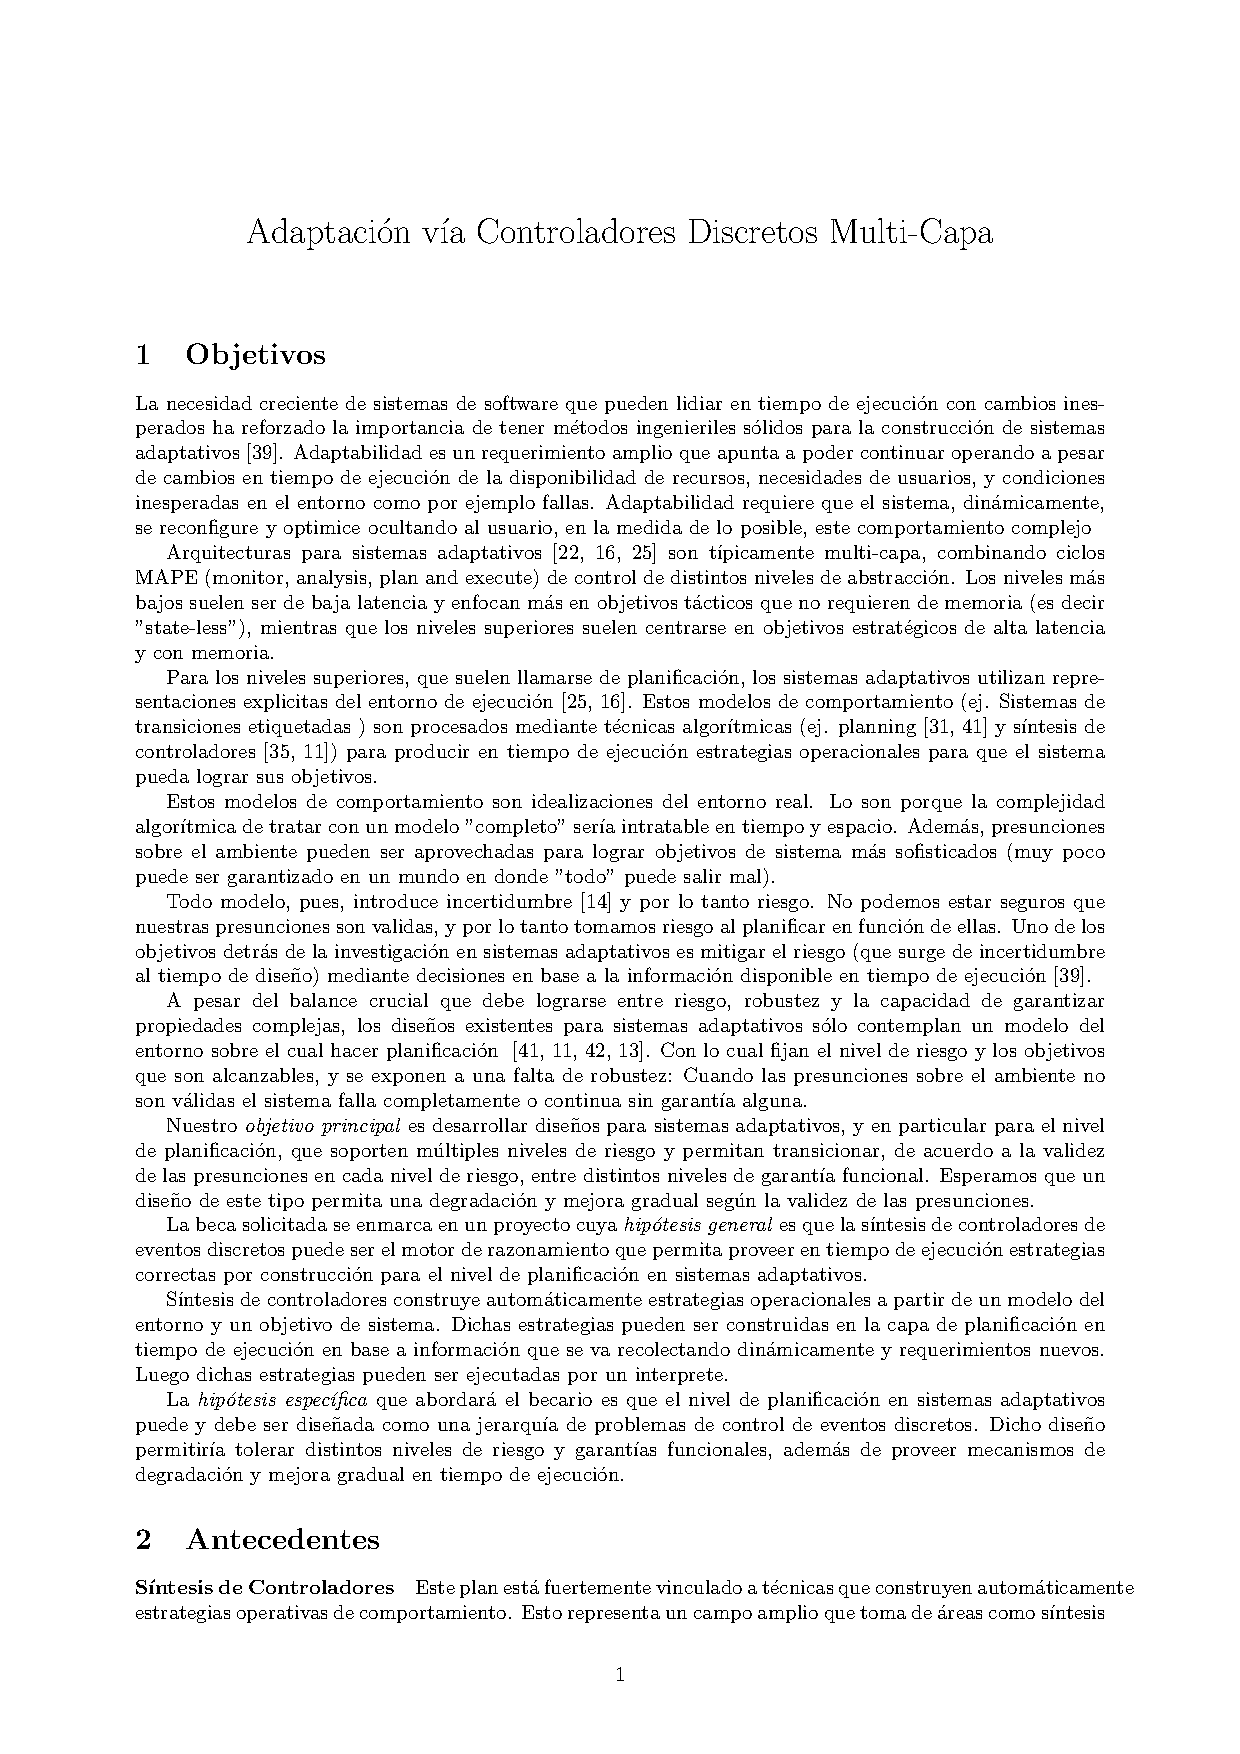
\includepdf[thread,pages=-]{plan-trabajo.pdf}
%%[]
%
%\textbf{Colaboradores involucrados en el plan de investigaci\'on}
%
%\begin{compactitem}
%\item Sebasti\'an Uchitel, FCEyN, UBA.
\item Nicol\'as D'Ippolito, FCEyN, UBA.
\item Victor Braberman, FCEyN, UBA.
\item Nir Piterman, Leicester University, Leicester, United Kingdom.
\item Jeff Kramer, Imperial College London, London, United Kingdom.
\item Kenji Tei, National Institute of Informatics.
\item Shinichi Honiden, National Institute of Informatics.

%\end{compactitem}
%
%\medskip
%
%\textbf{Plan de extensi�n}
%%%%%%%%%%%%
%
%Con respecto a la extensi\'on universitaria, planeo continuar
%colaborando con iniciativas tales como la ``Semana de la
%Computaci\'on'' o ``Cient\'{\i}ficos por un d\'{\i}a'', programas de
%interacci\'on con la escuela media que a mi juicio cumplen un
%importante rol en la divulgaci�n de las tareas de investigaci�n y
%docencia desarrolladas en el Departamento.
%
%
%%%fin plan de investigacion
%%
%%
%%%\firma

\end{document}
